\section{Inference Method}

\begin{frame}
	\frametitle{Specifications}
	
	\Large
	
	\begin{itemize}
		\item Where and how robots can travel is \textbf{fundamentally} defined by the
			  environment and its evolution over time
		\vspace{-0.5cm}
		\item A robot should \textbf{not collide} with entities in the environment
		\vspace{0.1cm}
		\item A robot should \textbf{smoothly navigate} throughout the entire environment
			  behaving as a ``\emph{human}''
		\vspace{0.1cm}
		\item Avoiding the \textbf{freezing problem}
	\end{itemize}
\end{frame}

\begin{frame}
	\frametitle{Requirements}
	
	\Large
	
	\begin{itemize}
		\item Realistic navigation in crowded spaces is an intrinsically
			  \emph{interactive} planning problem
		\vspace{0.1cm}
		\item Robots to be deployable in multiple environments
		\vspace{0.1cm}
		\item Efficient solution for platforms that have resource constraints
	\end{itemize}
\end{frame}

\begin{frame}
	\frametitle{Proposed Method}
	
	\large
	
	\vspace{0.2cm}
	
	\begin{block}{Idea}
		Simple parameterized motion model (based on the concept of \emph{Hybrid Reciprocal
		Velocity Obstacles}) that captures key elements of \textbf{how people navigate}
		when encountering other people in the same space; estimating the parameters of
		such a model from data
	\end{block}
	
	\begin{itemize}
		\item We conceptualize each other agent as adopting locally-optimal actions given
			  a potential goal
		\vspace{0.1cm}
		\item These goals, which drive movement intention, are of course latent and
			  unobserved by our planning agent
		\vspace{0.1cm}
		\item A planning agent infers from real-time noisy data these latent goals, and
			  then plan its own path accordingly
	\end{itemize}
\end{frame}

\begin{frame}
	\frametitle{Counterfactual Framework}
	
	\begin{center}
		\begin{tikzpicture}
			\node at (0,0) [draw=white,ultra thick,inner sep=0pt]
			{
				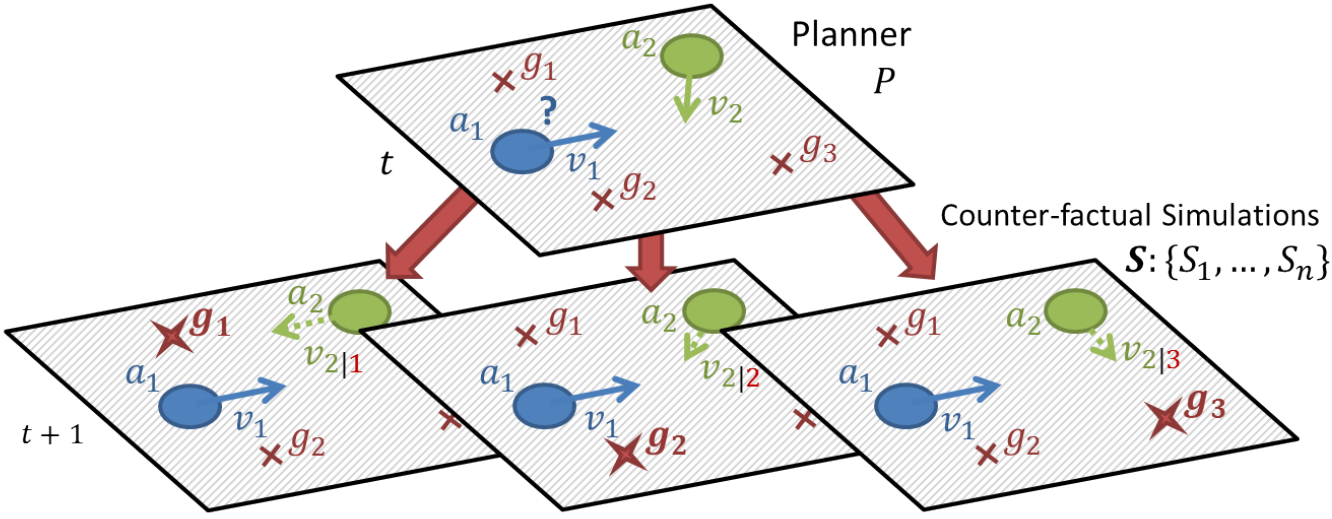
\includegraphics[scale=0.25]{Figures/CounterfactualFramework.png}
			};
		\end{tikzpicture}
	\end{center}
\end{frame}
